\documentclass[a4paper, 12pt]{article}

\usepackage{geometry}
\geometry{left=2cm, right=2cm, top=2cm, bottom=2cm}

\usepackage{cmap}
\usepackage{mathtext} 
\usepackage[T2A]{fontenc}
\usepackage[utf8]{inputenc}
\usepackage[english,russian]{babel}	

\usepackage{amsfonts,amssymb,amsthm,mathtools}
\usepackage{amsmath}
\usepackage{icomma} 

\usepackage{graphicx} 
\graphicspath{{picturies/}}
\usepackage{wrapfig}

\usepackage{array,tabularx,tabulary,booktabs}
\usepackage{longtable}
\usepackage{multirow}

\usepackage{caption}
\captionsetup{labelsep=period}

\renewcommand{\phi}{\varphi}
\newcommand{\eps}{\varepsilon}
\newcommand{\parag}[1]{\paragraph*{#1:}}

\newcounter{Points}
\setcounter{Points}{1}
\newcommand{\point}{\arabic{Points}. \addtocounter{Points}{1}}

\author{Радькин Кирилл, Б01-005}
\date{8.04.22}
\title{Лабораторная работа 4.7.3. Изучение поляризованного света.}
 
\begin{document}
\maketitle
\thispagestyle{empty}
\newpage

\textbf{Цель работы:} ознакомление с методами получения и анализа поляризованного света.
\\

\textbf{Оборудование:} оптическая скамья с осветителем; зелёный светофильтр; два поляроида; чёрное зеркало; полированная эбонитовая пластинка; стопа стеклянных пластинок; слюдяные пластинки разной толщины; пластинки в 1/4 и 1/2 длины волны; пластинка
в одну длину волны для зелёного света (пластинка чувствительного
оттенка).

\section{Теоретическая справка}
\subsection{Определение направления разрешённой плоскости колебаний поляроида}
	
	Определить направление разрешённых колебаний поляроида проще всего с помощью чёрного зеркала.
	
При падении на отражающую поверхность под углом Брюстера, свет в отражённом луче почти полностью поляризован, а вектор E параллелен отражающей поверхности. Луч света, прошедший поляроид и отразившийся от чёрного зеркала, имеет минимальную интенсивность при выполнении двух условий: свет падает на отражающую поверхность под углом Брюстера и вектор E лежит в плоскости падения.

Вращая поляроид вокруг направления луча и чёрное зеркало вокруг оси, перпендикулярной лучу, методом последовательных приближений можно добиться минимальной яркости луча, отражённого от зеркала, и таким образом определить разрешённое направление поляроида.

Измеряя угол поворота зеркала (угол Брюстера), нетрудно определить коэффициент преломления материала, из которого изготовлено зеркало. 

\subsection{Получение эллиптически поляризованного света}

Эллиптически поляризованный свет можно получить из линейно поляризованного с помощью двоякопреломляющих кристаллических пластинок.

Двоякопреломляющая пластинка имеет два взаимно перпендикулярных главных направления, совпадающих с осями эллипсоида диэлектрической проницаемости. Волны, поляризованные вдоль главных направлений, распространяются в пластинке с разными скоростями, не изменяя характера своей поляризации. Эти волны называются главными. Мы будем обозначать показатели преломления для главных волн через $ n_x $ и $ n_y $, где $ x $ и $ y $ --- главные направления кристаллической пластинки (Рис. $\ref{ris 1}$).
\begin{wrapfigure}{r}{0.4\linewidth}
	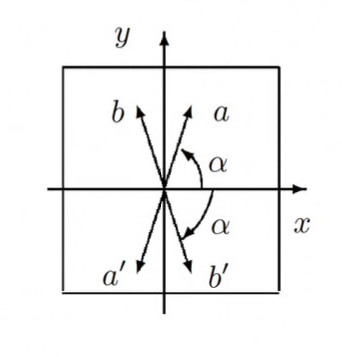
\includegraphics[width=\linewidth]{1.jpeg}
	\caption{Разложение линейно поляризованного света.}
	\label{ris 1}
\end{wrapfigure}


Пусть на пластинку падает линейно поляризованная волна, электрический вектор которой ориентирован под некоторым углом $ \alpha $ к оси
$ x $. Разложим вектор $ \mathbf{E} $ на составляющие $ E_x $ и $ E_y $. На входе пластинки $ E_x $ и $ E_y $ находятся в фазе. На выходе из-за разности скоростей между ними появляется разность хода $ d(n_x - n_y) $, при этом сдвиг фаз определяется соотношением

\begin{equation}\label{}
\Delta \phi =  \dfrac{2\pi}{m} = k d(n_x - n_y)
\end{equation}

Как уже отмечалось, при сложении двух взаимно перпендикулярных колебаний, обладающих некоторым сдвигом фаз, образуется колебание, поляризованное по эллипсу.



Рассмотрим практически важные частные случаи.

 \begin{enumerate}
 		
 	\item Пластинка даёт сдвиг фаз $ 2\pi $ (пластинка в длину волны $ \lambda $). В результате сложения волн на выходе пластинки образуется линейно поляризованная волна с тем же направлением колебаний, что и в падающей волне.

	\item Пластинка даёт сдвиг фаз $ \pi $ (пластинка в полдлины волны $ \lambda / 2 $). На выходе пластинки снова образуется линейно поляризованная волна. Направление $ bb' $ колебаний этой волны повёрнуто относительно направления $ aa' $ колебаний падающей волны (рис. 2). Как нетрудно сообразить, направление $ bb' $ является зеркальным отображением направления $ aa' $ относительно одного из главных направлений пластинки. Такую пластинку используют для поворота направления колебаний линейно поляризованного света.

 \end{enumerate}
 	
3.  Пластинка создаёт между колебаниями сдвиг фаз $ \pi/2 $ (пластинка
в четверть длины волны). При сложении двух взаимно перпендикулярных колебаний, имеющих разность фаз $ \pi/2 $, образуется эллипс, главные оси которого совпадают с координатными осями $ x $ и $ y $. При равенстве амплитуд возникает круговая поляризация.
 	


Следует отметить, что, говоря о пластинках $ \lambda , \lambda/2, \lambda/4  $ и т. д., всегда подразумевают какую-либо вполне определённую монохроматическую
компоненту (например, пластинка $ \lambda/2 $ для зелёного света). Если на двоякопреломляющую пластинку падает не монохроматический свет, то на
выходе из неё для разных спектральных компонент эллипсы поляризации будут различными.

\subsection{Анализ эллиптически поляризованного света}

Анализ эллиптически поляризованного света сводится к нахождению главных осей
эллипса поляризации и к определению направления вращения электрического вектора.

Главные оси эллипса поляризации определяются с помощью анализатора по максимуму и минимуму интенсивности проходящего света.
Направление вращения электрического вектора может быть найдено
с помощью пластинки в четверть длины волны, для которой известно,
какая из главных волн, $ E_x $ или $ E_y $, имеет б\'{o}льшую скорость распространения (и соответственно меньшее значение показателя преломления).

Выберем для определённости координатные оси x и y на пластинке
так, чтобы $ n_x < n_y $. В этом случае главная волна $ E_x $ имеет большую
скорость распространения. Поместим такую пластинку на пути эллиптически поляризованного света и совместим главные направления пластинки $ \lambda/4 $ с главными осями эллипса поляризации. На выходе из этой
пластинки сдвиг фаз между $ E_x $ и $ E_y $ вместо $ \pi/2 $ станет равным нулю или $ \pi $. Свет окажется линейно поляризованным. Из двух возможных значений сдвига фаз, 0 или $ \pi $, реализуется одно: то, которое соответствует имеющемуся в волне направлению вращения электрического вектора.

Рассмотрим, например, случай, когда электрический вектор в эллиптически поляризованной волне вращается против часовой стрелки,
если смотреть навстречу лучу. В этом случае, очевидно, в волне, падающей на пластинку в $ \lambda/4 $, колебание $ E_y $ отстаёт по фазе на $ \pi/2 $ от
колебания $ E_x $. При прохождении через пластинку разность фаз увеличивается до $ \pi $. Таким образом на выходе из пластинки возникают линейно поляризованные волны со сдвигом фаз $ \pi $. Сложение этих волн
даёт плоскополяризованную волну, электрический вектор которой располагается во втором и четвёртом квадрантах координатной системы
$ x, y $.

Рассуждая аналогичным образом, найдём, что при вращении электрического вектора по часовой стрелке направление колебаний в линейно поляризованной волне, выходящей из пластинки, располагается в первом и третьем квадрантах. Определяя направление колебаний на выходе из пластинки с помощью поляроида, можно, таким образом, определить характер эллиптической поляризации (вращение против или по часовой стрелке).

\subsection{Пластинка чувствительного оттенка}



Выше предполагалось известным, какому из двух главных направлений пластинки в четверть длины волны соответствует большая скорость распространения света.
Установить это можно различными способами, например с помощью
пластинки чувствительного оттенка (так называют пластинку в $ \lambda $
для зелёной спектральной компоненты, $ \lambda = 560 $ нм). Если пластинка чувствительного оттенка помещена между скрещенными поляроидами и главные направления пластинки не параллельны
направлениям разрешённых колебаний поляроидов, то при освещении
белым светом пластинка кажется окрашенной в лилово-красный цвет.
\begin{wrapfigure}{l}{0.35\linewidth}
	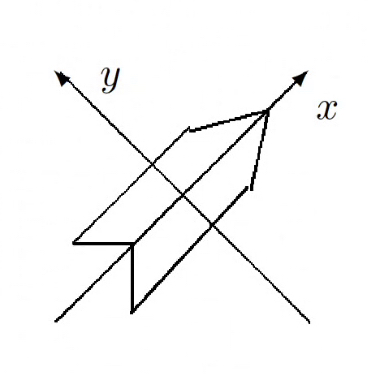
\includegraphics[width=\linewidth]{3}
	\caption{Пластинка чувствительного оттенка}
	\label{ris 3}
\end{wrapfigure}

Это объясняется тем, что зелёная компонента линейно поляризованного света при прохождении пластинки не меняет поляризации и задерживается вторым поляроидом. Для красной и фиолетовой компонент
пластинка создаёт сдвиг фаз, несколько отличный от $ 2\pi $. На выходе
из пластинки красная и фиолетовая компоненты оказываются поэтому
эллиптически поляризованными и частично проходят через второй поляроид. Таким образом, в известном смысле наблюдаемый в указанном
опыте цвет пластинки дополнителен к зелёному.

Если между скрещенными поляроидами поместить пластинку чувствительного оттенка
($ \lambda $) и пластинку в $ \lambda/4 $ так, чтобы их главные
направления совпадали, цвет пластинки изменится. Если у пластинки чувствительного оттенка и пластинки в $ \lambda/4 $ совпадут главные направления, соответствующие большей скорости распространения, то разность хода между $ E_x $ и $ E_y $ для зелёного света составит уже $ 5\lambda/4 $. Это соответствует разности хода в $ \lambda $ для света с большей длиной волны, т. е. для "<более красного"> света. При освещении
этих пластинок (напомним, что они расположены между скрещенными поляроидами) белым светом теперь погасится не зелёная, а красная
часть спектра, и проходящий свет будет казаться зеленовато-голубым.
Если же главные направления, соответствующие большей скорости распространения, у пластинки чувствительного оттенка и у пластинки
в $ \lambda/4 $ окажутся перпендикулярными, то проходящий свет приобретёт
оранжево-желтую окраску (погасится фиолетово-голубая часть спектра).

Изменение цвета позволяет, таким образом, определить, какое из
главных направлений пластинки в $ \lambda/4 $ соответствует большей скорости
распространения.

\subsection{Интерференция поляризованных лучей}

\begin{figure}{}
	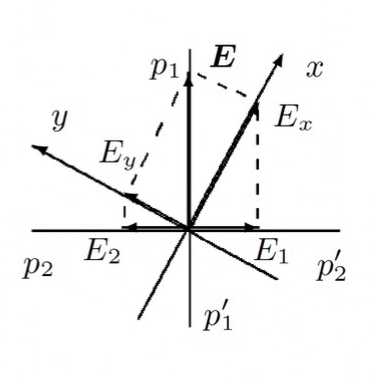
\includegraphics[scale=0.7]{4}
	\centering
	\caption{К объяснению интерференции
поляризованных лучей}
	\label{ris 4}
\end{figure}


Тонкие двоякопреломляющие пластинки, помещённые между поляроидами, кажутся окрашенными. Эта окраска может быть истолкована как результат интерференции поляризованных лучей. На рис. 4 представлена схема для
случая скрещенных поляроидов.

Здесь $ p_1p'_1 $ --- разрешённое направление колебаний поляризатора
(первого поляроида); $ x, y $ --- координатная система, связанная с главны-
ми направлениями двоякопреломляющей пластинки; $ p_2p'_2 $ --- разрешённое направление колебаний анализатора (второго поляроида). Волны
$ E_x  $ и $ E_y $ на выходе из пластинки когерентны, но не могут интерферировать, так как $ E_x \perp  E_y $. Волны $ E_1 $ и $ E_2 $ на выходе второго поляроида
также являются когерентными и к тому же поляризованы в одной плоскости. Эти волны интерферируют между собой. Результат интерференции определяется зависящим от длины волны сдвигом фаз между $ E_1 $
и $ E_2 $. В результате интерференции поляризованных лучей пластинка, освещаемая белым светом, кажется окрашенной.

Если поворачивать двоякопреломляющую пластинку, расположенную между
скрещенными поляроидами, то соотношение амплитуд волн $ E_1 $ и $ E_2 $ и разность фаз между ними не изменяются. Это означает, что цвет пластинки при её поворотах не меняется, а меняется только интенсивность света. За один оборот пластинки интенсивность четыре раза обращается в нуль --- это происходит при совпадении главных направлений
$ x $ и $ y $ с разрешёнными направлениями колебаний поляроидов.

\section{Ход работы}
\subsection{Определение разрешенных направлений поляроида}

\begin{wrapfigure}{r}{0.35\linewidth}
	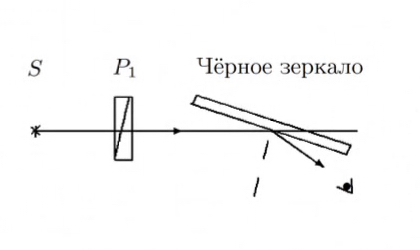
\includegraphics[width=\linewidth]{5}
	\caption{Определение разрешенных направлений поляроида}
	\label{ris 5}
\end{wrapfigure}

Поворачивая поляроид вокруг направления луча, добъемся наименьшей яркости отражённого пятна. Оставим поляроид в этом положении и вращением зеркала вокруг вертикальной оси снова добъемся минимальной интенсивности отражённого луча. Уточним положения поляроида
и зеркала, соответствующие минимуму интенсивности, и определим разрешённое направление поляроида: $8^\circ$.

Разрешённое направление второго поляроида можно определить, скрестив поляроиды: после поляроида с известной поляризацией поставим второй поляроид и, глядя навстречу лучу, вращением второго поляроида добъемся минимальной яркости луча. Разрешенное направление второго поляроида: $-10^\circ$

\subsection{Определение показателя преломления эбонита}

Поставим на скамью вместо чёрного зеркала (Рис. $\ref{ris 5}$) эбонитовую
пластину и определим по лимбу угол Брюстера. Получаем $ \theta_1 =(58 \pm 5) ^\circ$ без фильтра и $ \theta_2 =(56 \pm 5) ^\circ$. 

Отсюда получаем, что $ n = \tg \theta_1 \approx 1.6 \pm 0.2 $. Табличное значение коэффициента преломления эбонита находится между 1.6 и 1.7.

\subsection{Исследование стопы}

\begin{wrapfigure}{l}{0.35\linewidth}
	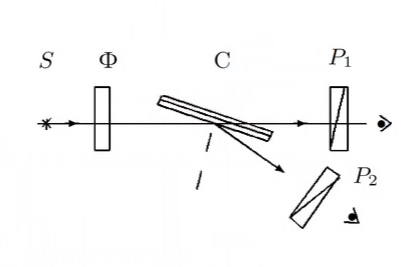
\includegraphics[width=\linewidth]{6}
	\caption{Исследование стопы}
	\label{ris 6}
\end{wrapfigure}

Исследуем характер поляризации света в преломлённом и отражённом от стопы лучах. 

Для этого поставим вместо эбонитового зеркала (Рис. $\ref{ris 6}$) стопу стеклянных пластинок под углом Брюстера.

В отраженном луче минимум при $5^\circ$ на поляризаторе $\rightarrow$ у отраженного луча поляризация вертикальная. В преломленном луче при $98^\circ$ минимум $\rightarrow$ поляризация горизонтальная.
\\\\\\

\subsection{Двоякопреломляющие пластины}
\begin{wrapfigure}{l}{0.35\linewidth}
	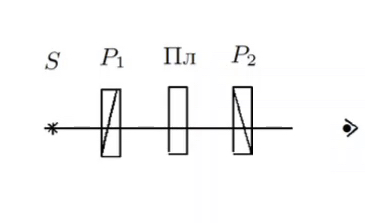
\includegraphics[width=\linewidth]{7}
	\caption{Определение главных
		направлений в пластинках}
	\label{ris 7}
\end{wrapfigure}

Поставим однородную кристаллическую пластинку между скрещенными поляроидами. Вращая пластинку вокруг направления луча и наблюдая за интенсивностью света, проходящего сквозь второй поляроид, определим, при каком условии главные направления пластинки совпадают с разрешёнными направлениями поляроидов.

У первой пластины: $277^\circ$~---~горизонтальное направление, у второй пластинки: $5^\circ$~---~горизонтальное направление.

\subsection{Пластинки $ \lambda/2, \lambda/4 $}

Для выделения пластин $ \lambda/2, \lambda/4 $ Добавим к схеме, изображённой на Рис. $\ref{ris 8}$, зелёный фильтр и установим разрешённое направление первого поляроида горизонтально, а главные направления исследуемой пластинки --- под углом $ 45^\circ $ к горизонтали.

C помощью второго поляроида установим, какую поляризацию имеет свет, прошедший пластинку: круговую или линейную. В случае пластинки $ \lambda/4 $ получаем круговую поляризацию, а при $ \lambda/2 $~---~линейную.

\newpage

\subsection{Быстрая и медленная оси $ \lambda/4 $}

\begin{wrapfigure}{r}{0.35\linewidth}
	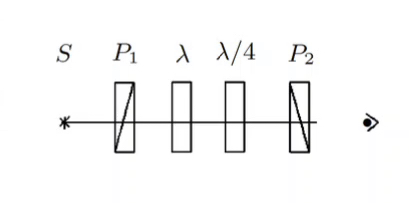
\includegraphics[width=\linewidth]{8}
	\caption{Определение направлений
большей и меньшей скорости}
	\label{ris 8}
\end{wrapfigure}

Поставим между скрещенными поляроидами пластинку чувствительного оттенка, имеющую вид стрелки. Уберем зелёный фильтр и убедимся, что стрелка имеет пурпурныйцвет. Это объясняется тем, что зелёная компонента линейно поляризованного света при прохождении пластинки не меняет поляризации и задерживается вторым поляроидом. 
Добавим к схеме пластинку $ \lambda/4 $ (Рис. $\ref{ris 8}$), главные направления которой совпадают с главными направлениями пластины $ \lambda $ и ориентированы под углом $ 45^\circ $ к разрешённым направлениям скрещенных поляроидов. При повороте рейтера со стрелкой на $ 180^\circ $ вокруг вертикальной оси цвет стрелки меняется от зелёно-голубого до оранжево-жёлтого. В первом случае у нас "<быстрая"> ось (они совпадают), во втором --- медленная согласно пункту 1.4.

\subsection{Эллиптически поляризованная волна}

Нарисуем эллипс поляризации для вектора напряжённости из пластинки $ \lambda/4 $ и укажем, какая из осей соответствует большей скорости. Это ось $ x $. Рядом нарисуем две вышедших из пластинки синусоиды: $ x(t) $ (красная) и $ y(t) $ (синяя) со сдвигом фаз в четверть периода. Определим направление вращения электрического вектора в эллиптически поляризованной волне.

\begin{figure}[!h]
	\begin{minipage}{0.48\linewidth}
		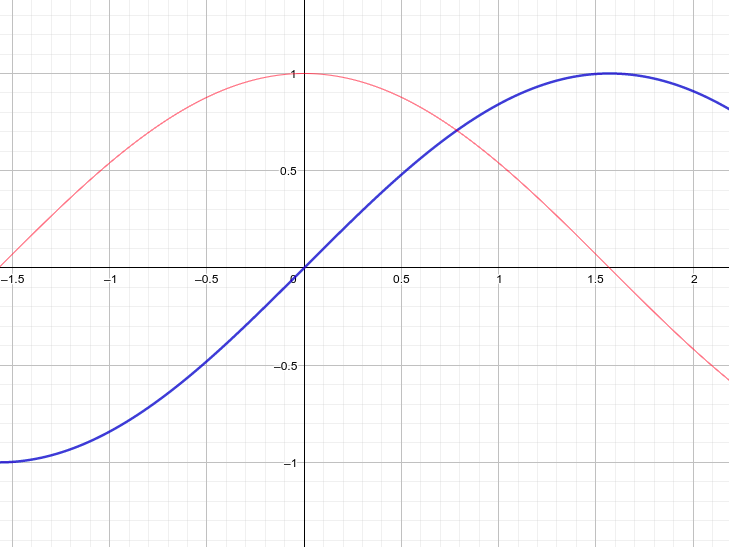
\includegraphics[width=\linewidth]{image1.png}
		\centering
		\caption{Синусоиды со свдигом фаз $\pi/2$}
	\end{minipage}
	\hfill
	\begin{minipage}{0.49\linewidth}
		\centering
		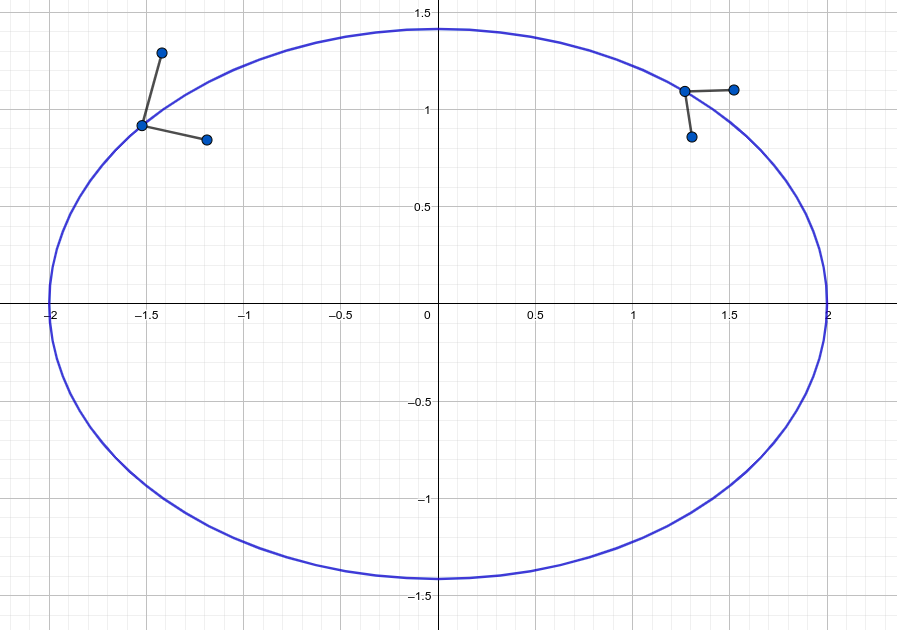
\includegraphics[width=\linewidth]{ellips.png}
		\caption{Эллипс поляризации}
	\end{minipage}
\end{figure}

Т.к. на выходе вектор $E$ остался в 1-3 квадрантах, это означает, что вращение происходит против часововй стрелки.

\subsection{Интерференция поляризованных лучей}

Исследуем интерференцию поляризованных лучей. Для этого расположим между скрещенными поляроидами мозаичную слюдяную пластинку. Она собрана из 4-х узких полосок слюды, лежащих по сторонам квадрата (две полоски "<толщиной"> $ \lambda/4 $ и по одной --- $ \lambda/2 $ и $ 3\lambda/4 $). В центральном квадратике слюды нет. Главные направления всех пластинок ориентированы параллельно сторонам квадрата.
При вращении пластинки изменяются только цвета в ячейках (кроме центральной). При вращении поляроида меняются цвет и интенсивность света в клетках.


\end{document}